\chapter{Evaluation}

\section{Introduzione}
In questo capitolo, esamineremo i risultati ottenuti dalla \textbf{validazione incrociata} (\textbf{K-fold cross-validation}) sui modelli di classificazione \textbf{Naive Bayes} e \textbf{Support Vector Machine} (\textbf{SVM}). L'obiettivo principale è valutare le prestazioni di ciascun modello in modo sistematico e approfondito, utilizzando un approccio rigoroso basato su \textbf{metriche quantitative}.

Per ottenere un'analisi dettagliata, misureremo le performance di entrambi i modelli attraverso metriche chiave come \textbf{accuratezza}, \textbf{matrice di confusione}, \textbf{precisione}, \textbf{recall}, \textbf{F1-score} e \textbf{overfitting}. La \textbf{validazione incrociata} consente di ridurre la variabilità nei risultati e garantire che le \textbf{prestazioni osservate} non dipendano da una particolare suddivisione dei dati. In questo contesto, il \textbf{confronto} tra Naive Bayes e SVM permetterà di evidenziare differenze significative in termini di \textbf{capacità predittiva}, \textbf{robustezza} e \textbf{adattabilità} a differenti \textbf{distribuzioni dei dati}.

Infine, discuteremo dei possibili \textbf{scenari applicativi} in cui ciascun modello potrebbe risultare più adatto, considerando fattori come la \textbf{sensibilità ai dati sbilanciati}, le \textbf{risorse computazionali richieste} e l'\textbf{interpretabilità del modello}.



\section{Metriche di Valutazione dei Modelli}
Per valutare le prestazioni dei modelli, sono state utilizzate le seguenti metriche:

\begin{itemize}
    \item \textbf{Accuratezza}: misura la percentuale di previsioni corrette rispetto al numero totale di previsioni.
    \begin{equation} Accuracy = \frac{TP+TN}{TP+TN+FP+FN}\end{equation}

    \item \textbf{Precisione} (o \textbf{Positive Predictive Value}): indica la percentuale di previsioni positive corrette rispetto a tutte le previsioni positive fatte dal modello.
    \begin{equation} Precision = \frac{TP}{TP+FP}\end{equation}

    \item \textbf{Recall} (o \textbf{Sensibilità} o \textbf{True Positive Rate}): misura la percentuale di veri positivi identificati correttamente dal modello.
    \begin{equation} Recall = \frac{TP}{TP+FN}\end{equation}

    \item \textbf{F1-score}: è la media armonica di precisione e recall, che bilancia entrambi i valori. È utile quando c'è uno squilibrio tra le classi.\begin{equation} F1 = \frac{2*Precision*Recall}{Precision+Recall}\end{equation}

    \item \textbf{Overfitting}: misura la differenza tra l'accuratezza sui dati di addestramento e l'accuratezza sui dati di test per valutare la capacit\`a di generalizzazione del modello. Un valore elevato di questa differenza indica che il modello si adatta troppo ai dati di training e potrebbe non generalizzare bene su dati non visti.\begin{equation}Overfitting = Accuracy_{train} - Accuracy_{test}\end{equation}
\end{itemize}

Dove:
\begin{itemize}
    \item \textbf{TP} è il numero di veri positivi,
    \item \textbf{TN} è il numero di veri negativi,
    \item \textbf{FP} è il numero di falsi positivi,
    \item \textbf{FN} è il numero di falsi negativi.
\end{itemize}

\newpage

\section{Risultati del Modello Naive Bayes}

\subsection{Risultati di Addestramento}

Il modello \textbf{Naive Bayes} ha ottenuto un'accuratezza complessiva del \textbf{92.87\%} sui dati di addestramento. Questa performance suggerisce una buona capacità del modello di generalizzare il comportamento delle classi, mantenendo un buon livello di prestazioni anche su dati non visti. \\ \\
La matrice di confusione, che riporta il numero di previsioni corrette e errate per ciascuna classe, mostra i seguenti risultati:

\begin{figure}[H]
    \centering
    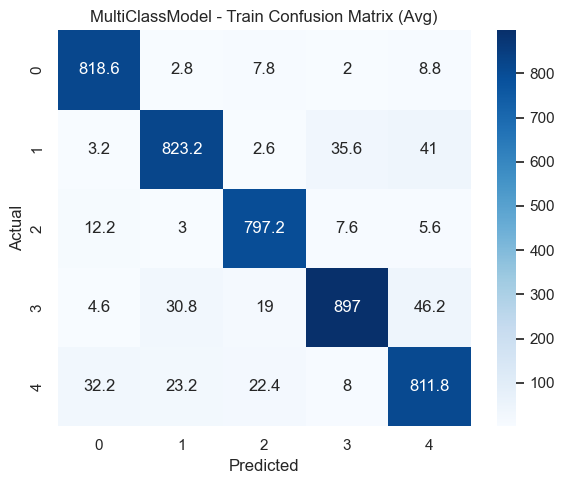
\includegraphics[width=0.8\textwidth]{images/confusion_matrix_train_naive_bayes.png}
    \caption{Matrice di confusione per il training di Naive Bayes}
    \label{fig:confusion_matrix_train_naive_bayes}
\end{figure}

Il modello mostra buone prestazioni complessive, con un'alta percentuale di istanze correttamente classificate, come evidenziato dai valori elevati sulla \textbf{diagonale principale}. Tuttavia, ci sono errori significativi tra alcune classi, in particolare tra le classi 1, 3 e 4, dove il modello ha difficoltà a distinguere correttamente. Questo evidenzia alcune aree in cui il modello potrebbe migliorare nel riconoscere meglio le differenze tra queste classi.

\newpage

Le metriche per ogni categoria sono mostrate nella seguente tabella e visualizzate nel seguente grafico:

\begin{table}[H]
    \centering
    \begin{tabular}{|c|c|c|c|c|}
        \hline
        \textbf{Categoria} & \textbf{Precision} & \textbf{Recall} & \textbf{F1-score} \\
        \hline
        Accesso & 94.01\% & 97.45\% & 95.70\% \\
        \hline
        Didattica & 93.23\% & 90.90\% & 92.05\% \\
        \hline
        Profilo & 93.90\% & 96.56\% & 95.21\% \\
        \hline
        Segreteria & 94.40\% & 89.91\% & 92.10\% \\
        \hline
        Tecnico & 88.89\% & 90.44\% & 89.65\% \\
        \hline
        media & 93.27\% & 93.28\% & 93.27\% \\
        \hline
        media pesata & 93.16\% & 93.16\% & 93.16\% \\
        \hline
    \end{tabular}
    \caption{Confronto tra precision, recall e F1-score per il training di Naive Bayes}
    \label{tab:metriche_naive_bayes_train}
\end{table}

\begin{figure}[H]
    \centering
    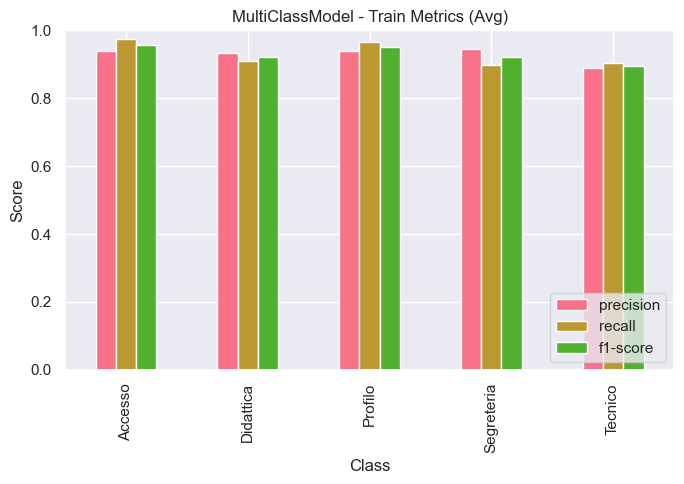
\includegraphics[width=0.8\textwidth]{images/metrics_train_naive_bayes.png}
    \caption{Confronto tra precision, recall e F1-score per il training di Naive Bayes}
    \label{fig:metrics_train_naive_bayes}
\end{figure}

Il modello mostra buone performance complessive, ma nelle categorie \textbf{Segreteria} e \textbf{Tecnico} ci sono margini di miglioramento. \textbf{Segreteria} ha alta precisione ma basso richiamo, mentre \textbf{Tecnico} ha alta capacità di identificare le istanze (buon richiamo), ma con una precisione più bassa. Queste discrepanze suggeriscono che il modello può essere ottimizzato per bilanciare meglio precisione e richiamo in queste categorie.

\newpage

\subsection{Risultati di Test}

Per quanto riguarda i \textbf{dati di test}, il modello ha ottenuto un'accuratezza del \textbf{89.74\%}, una leggera riduzione rispetto ai dati di addestramento, ma comunque una performance robusta. \\ \\
La matrice di confusione sui dati di test è la seguente:

\begin{figure}[H]
    \centering
    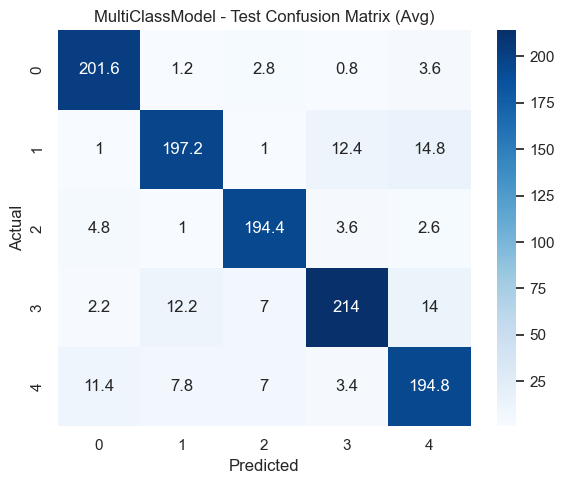
\includegraphics[width=0.8\textwidth]{images/confusion_matrix_test_naive_bayes.png}
    \caption{Matrice di confusione per il testing di Naive Bayes}
    \label{fig:confusion_matrix_test_naive_bayes}
\end{figure}

Mentre le metriche per ogni categoria sono mostrate nella seguente tabella e visualizzate nel seguente grafico:

\begin{table}[H]
    \centering
    \begin{tabular}{|c|c|c|c|c|}
        \hline
        \textbf{Categoria} & \textbf{Precision} & \textbf{Recall} & \textbf{F1-score} \\
        \hline
        Accesso & 91.29\% & 96.01\% & 93.56\% \\
        \hline
        Didattica & 89.92\% & 87.10\% & 88.47\% \\
        \hline
        Profilo & 91.59\% & 94.20\% & 92.87\% \\
        \hline
        Segreteria & 91.33\% & 85.78\% & 88.46\% \\
        \hline
        Tecnico & 84.76\% & 86.88\% & 85.80\% \\
        \hline
        media & 89.78\% & 89.79\% & 89.71\% \\
        \hline
        media pesata & 89.79\% & 89.74\% & 89.71\% \\
        \hline
    \end{tabular}
    \caption{Confronto tra precision, recall e F1-score per il testing di Naive Bayes}
    \label{tab:metriche_naive_bayes_test}
\end{table}

\begin{figure}[H]
    \centering
    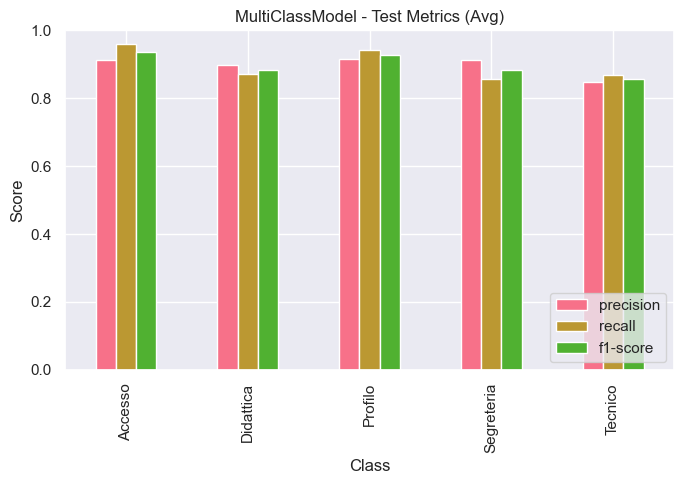
\includegraphics[width=0.8\textwidth]{images/metrics_test_naive_bayes.png}
    \caption{Confronto tra precision, recall e F1-score per il testing di Naive Bayes}
    \label{fig:metrics_test_naive_bayes}
\end{figure}

\subsection{Overfitting}

Per valutare il rischio di \textbf{overfitting}, sono stati analizzati i valori di accuratezza nei diversi fold della validazione incrociata a k-fold. Le differenze tra l'accuratezza dei dati variano tra \textbf{0.02} e \textbf{0.04}, con una media di \textbf{0.0313}. Sebbene vi sia una leggera tendenza all'overfitting, i valori rientrano in un intervallo accettabile, confermando la buona generalizzazione del modello.

\begin{figure}[H]
    \centering
    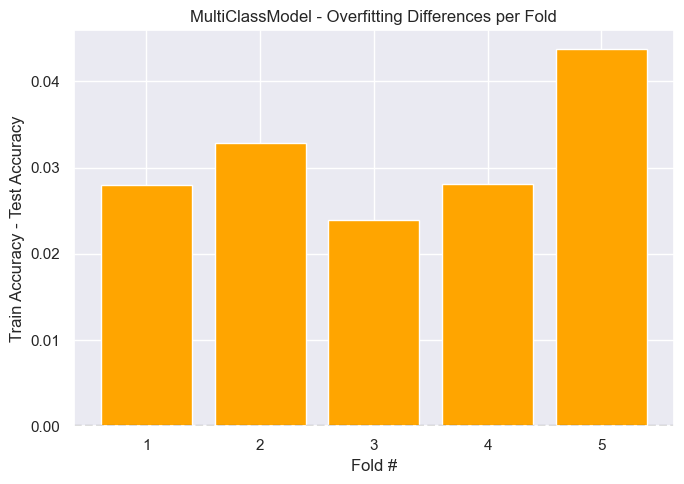
\includegraphics[width=0.8\textwidth]{images/overfitting_naive_bayes.png}
    \caption{Confronto dell'overfitting nei 5 fold per Naive Bayes}
    \label{fig:overfitting_naive_bayes}
\end{figure}

\newpage

\section{Risultati del Modello Support Vector Machine (SVM)}

\subsection{Risultati di Addestramento}

Il modello \textbf{Support Vector Machine (SVM)} ha ottenuto un'accuratezza complessiva del \textbf{93.17\%} sui dati di addestramento. Questo risultato suggerisce una forte capacità del modello nel generalizzare il comportamento delle classi, mantenendo alte prestazioni anche su dati non visti. \\ \\
La matrice di confusione, che riporta il numero di previsioni corrette ed errate per ciascuna classe, è la seguente:

\begin{figure}[H]
    \centering
    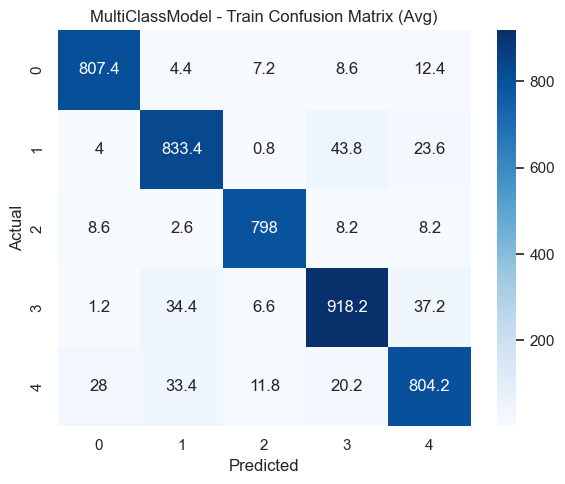
\includegraphics[width=0.8\textwidth]{images/confusion_matrix_train_svm.png}
    \caption{Matrice di confusione per i dati di addestramento con SVM}
    \label{fig:confusion_matrix_train_svm}
\end{figure}

Il modello mostra buone prestazioni complessive, con un’alta percentuale di istanze correttamente classificate, come evidenziato dai valori elevati sulla \textbf{diagonale principale}. Tuttavia, ci sono errori notabili tra alcune classi, in particolare tra le classi 1 e 4, dove il modello fatica a distinguere correttamente. Questo evidenzia alcune aree in cui il modello potrebbe migliorare nel riconoscere meglio le differenze tra queste classi.

\newpage

Le metriche per ogni categoria sono mostrate nella seguente tabella e visualizzate nel seguente grafico:

\begin{table}[H]
    \centering
    \begin{tabular}{|c|c|c|c|c|}
        \hline
        \textbf{Categoria} & \textbf{Precision} & \textbf{Recall} & \textbf{F1-score} \\
        \hline
        Accesso & 95.08\% & 96.12\% & 95.59\% \\
        \hline
        Didattica & 91.77\% & 92.02\% & 91.89\% \\
        \hline
        Profilo & 96.80\% & 96.65\% & 96.73\% \\
        \hline
        Segreteria & 91.92\% & 92.04\% & 91.98\% \\
        \hline
        Tecnico & 90.82\% & 89.60\% & 90.20\% \\
        \hline
        media & 93.28\% & 93.29\% & 93.28\% \\
        \hline
        media pesata & 93.16\% & 93.17\% & 93.16\% \\
        \hline
    \end{tabular}
    \caption{Confronto tra precision, recall e F1-score per il training di SVM}
    \label{tab:metriche_svm_train}
\end{table}

\begin{figure}[H]
    \centering
    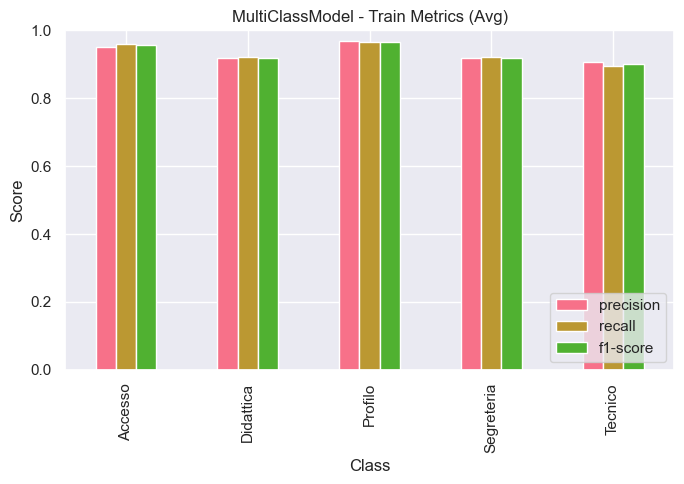
\includegraphics[width=0.8\textwidth]{images/metrics_train_svm.png}
    \caption{Confronto tra precision, recall e F1-score per il training di SVM}
    \label{fig:metrics_train_svm}
\end{figure}

Il modello ha buone performance complessive, ma nelle categorie \textbf{Tecnico} e \textbf{Didattica} ci sono margini di miglioramento. \textbf{Tecnico} mostra un buon richiamo, ma una precisione relativamente bassa, mentre \textbf{Didattica} ha una buona precisione, ma un richiamo leggermente inferiore. Queste discrepanze indicano che il modello potrebbe essere ottimizzato per migliorare l'equilibrio tra precisione e richiamo in queste categorie.

\newpage

\subsection{Risultati di Test}

Per quanto riguarda i \textbf{dati di test}, il modello ha ottenuto un'accuratezza del \textbf{90.79\%}, con una leggera riduzione rispetto ai dati di addestramento, ma comunque una performance robusta. \\ \\
La matrice di confusione sui dati di test è la seguente:

\begin{figure}[H]
    \centering
    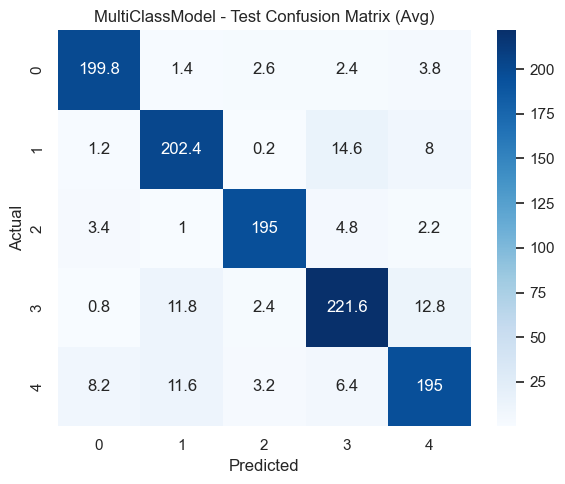
\includegraphics[width=0.8\textwidth]{images/confusion_matrix_test_svm.png}
    \caption{Matrice di confusione per i dati di test con SVM}
    \label{fig:confusion_matrix_test_svm}
\end{figure}

Mentre le metriche per ogni categoria sono mostrate nella seguente tabella e visualizzate nel seguente grafico:

\begin{table}[H]
    \centering
    \begin{tabular}{|c|c|c|c|c|}
        \hline
        \textbf{Categoria} & \textbf{Precision} & \textbf{Recall} & \textbf{F1-score} \\
        \hline
        Accesso & 93.66\% & 95.14\% & 94.37\% \\
        \hline
        Didattica & 88.72\% & 89.42\% & 89.06\% \\
        \hline
        Profilo & 95.89\% & 94.45\% & 95.16\% \\
        \hline
        Segreteria & 88.68\% & 88.82\% & 88.74\% \\
        \hline
        Tecnico & 87.94\% & 86.96\% & 87.43\% \\
        \hline
        media & 90.98\% & 90.96\% & 90.95\% \\
        \hline
        media pesata & 90.81\% & 90.79\% & 90.79\% \\
        \hline
    \end{tabular}
    \caption{Confronto tra precision, recall e F1-score per il testing di SVM}
    \label{tab:metriche_svm_test}
\end{table}

\begin{figure}[H]
    \centering
    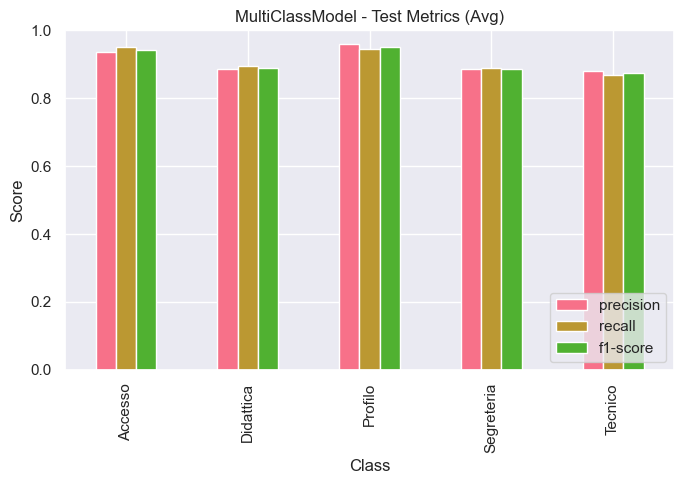
\includegraphics[width=0.8\textwidth]{images/metrics_test_svm.png}
    \caption{Confronto tra precision, recall e F1-score per il testing di SVM}
    \label{fig:metrics_test_svm}
\end{figure}

\subsection{Overfitting}

Per valutare il rischio di \textbf{overfitting}, sono stati analizzati i valori di accuratezza nei diversi fold della validazione incrociata a k-fold. Le differenze tra l'accuratezza dei dati variano tra \textbf{0.02} e \textbf{0.04}, con una media di \textbf{0.0237}. Sebbene ci sia una leggera tendenza all'overfitting, i valori rientrano in un intervallo accettabile, confermando la buona generalizzazione del modello.

\begin{figure}[H]
    \centering
    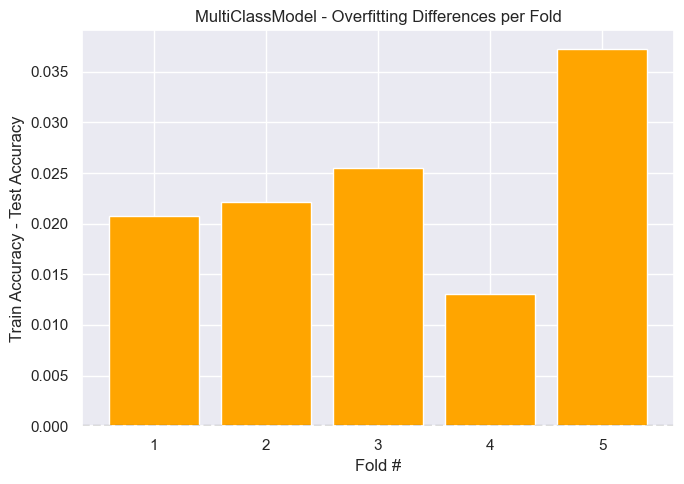
\includegraphics[width=0.8\textwidth]{images/overfitting_svm.png}
    \caption{Confronto dell'overfitting nei 5 fold per SVM}
    \label{fig:overfitting_svm}
\end{figure}

\newpage

\section{Confronto tra i Modelli}

\subsection{Prestazioni Complessive}

Entrambi i modelli, \textbf{Naive Bayes} e \textbf{SVM}, mostrano prestazioni molto simili. Durante il training, \textbf{Naive Bayes} raggiunge un'accuratezza del 92.87\%, mentre \textbf{SVM} è leggermente migliore con un'accuratezza del 93.17\%. Quando testati sui dati di test, entrambi i modelli registrano una piccola diminuzione delle performance, con \textbf{Naive Bayes} che scende al 89.74\% e \textbf{SVM} che ottiene il 90.79\%. Le metriche di precisione, recall e f1-score sono anch'esse molto simili per entrambi i modelli, suggerendo che entrambi sono abbastanza equilibrati nel bilanciare la capacità di classificare correttamente le istanze e nel ridurre al minimo gli errori.

\begin{table}[H]
    \centering
    \begin{tabular}{|c|c|c|c|c|c|}
        \hline
        \textbf{Modello} & \textbf{Set} & \textbf{Accuracy} & \textbf{Precision} & \textbf{Recall} & \textbf{F1-score} \\
        \hline
        Naive Bayes & Training & 92.87\% & 93.29\% & 92.91\% & 92.88\% \\
        \hline
        Naive Bayes & Test & 89.74\% & 89.91\% & 89.80\% & 89.79\% \\
        \hline
        SVM & Training & 93.17\% & 93.16\% & 93.21\% & 93.16\% \\
        \hline
        SVM & Test & 90.79\% & 90.82\% & 90.85\% & 90.79\% \\
        \hline
    \end{tabular}
    \caption{Confronto tra i modelli in termini di accuracy, precision, recall e F1-score}
    \label{tab:confronto_metriche}
\end{table}


\subsection{Overfitting}

Sia il modello \textbf{Naive Bayes} che il modello \textbf{SVM} mostrano una lieve presenza di \textbf{overfitting}, con differenze tra le performance sui dati che variano tra \textbf{0.02} e \textbf{0.04}. \\ \\
Per meglio visualizzare e comprendere l'andamento dell'overfitting, è stato calcolato il valore della differenza per ogni fold del k-fold cross-validation. La seguente immagine mostra queste differenze per ciascun fold, confrontando l'overfitting tra i modelli Naive Bayes e SVM.

\begin{figure}[H]
    \centering
    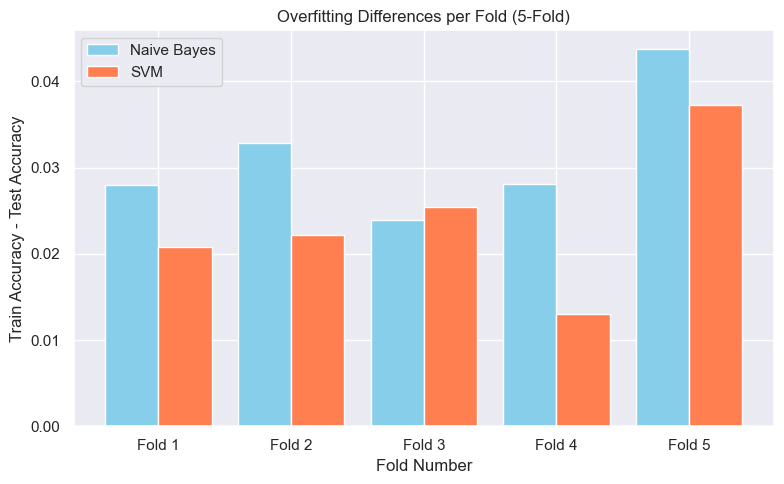
\includegraphics[width=0.8\textwidth]{images/overfitting_differences.png}
    \caption{Confronto dell'overfitting tra Naive Bayes e SVM}
    \label{fig:overfitting_differences}
\end{figure}

\section{Conclusioni}

Entrambi i modelli, Naive Bayes e Support Vector Machine (SVM), hanno mostrato prestazioni eccellenti nel compito di \textbf{classificazione}, evidenziando differenze minime nelle metriche di valutazione. Sebbene il modello SVM ottenga leggermente migliori risultati in termini di accuratezza sui dati di test, con un'accuratezza del \textbf{90.79\%} rispetto al \textbf{89.74\%} di Naive Bayes, la differenza tra i due modelli risulta essere piuttosto contenuta, con un margine di soli pochi punti percentuali. Questo indica che entrambi i modelli sono ben calibrati per il compito e sono capaci di generalizzare efficacemente anche su dati non visti.

\textbf{Naive Bayes}, grazie alla sua semplicità e velocità di esecuzione, potrebbe essere la scelta preferibile in scenari in cui le risorse computazionali sono limitate o in situazioni che richiedono modelli facilmente interpretabili. Inoltre, la capacità di Naive Bayes di gestire efficacemente grandi volumi di dati con risorse relativamente basse lo rende adatto per applicazioni in tempo reale o su dispositivi con risorse limitate.

D'altra parte, il modello \textbf{SVM} si distingue per una maggiore precisione in alcuni casi, come evidenziato dalle metriche di precisione e recall, ed è generalmente considerato una scelta solida quando è necessaria una maggiore accuratezza, specialmente in contesti dove la performance sui dati di test è cruciale e si dispone di risorse computazionali adeguate. SVM è inoltre più adatto per situazioni che richiedono una maggiore capacità di generalizzazione rispetto a modelli con assunzioni più forti, come Naive Bayes.

In definitiva, entrambi i modelli sono validi per il problema in esame e presentano un buon compromesso tra \textbf{accuratezza} e capacità di \textbf{generalizzazione}. La scelta finale tra Naive Bayes e SVM dipenderà da considerazioni specifiche relative all'ambiente applicativo, come la disponibilità di risorse computazionali, la necessità di interpretabilità del modello e la priorità data a una leggera miglioria nelle prestazioni rispetto alla velocità di esecuzione.




